\documentclass[12pt,letterpaper]{article}
\usepackage[utf8]{inputenc}
\usepackage[spanish]{babel}
\usepackage{graphicx}
\usepackage[left=2cm,right=2cm,top=2cm,bottom=2cm]{geometry}
\usepackage{graphicx} % figuras
% \usepackage{subfigure} % subfiguras
\usepackage{float} % para usar [H]
\usepackage{amsmath}
%\usepackage{txfonts}
\usepackage{stackrel} 
\usepackage{multirow}
\usepackage{enumerate} % enumerados
\renewcommand{\labelitemi}{$-$}
\renewcommand{\labelitemii}{$\cdot$}
% \author{}
% \title{Caratula}
\begin{document}

% Fancy Header and Footer
% \usepackage{fancyhdr}
% \pagestyle{fancy}
% \cfoot{}
% \rfoot{\thepage}
%

% \usepackage[hidelinks]{hyperref} % CREA HYPERVINCULOS EN INDICE

% \author{}
\title{Caratula}

\begin{titlepage}
\begin{center}
\large{UNIVERSIDAD PRIVADA-DE-TACNA}\\
\vspace*{-0.025in}
\begin{figure}[htb]
\begin{center}

\includegraphics[width=8cm]{./Imagenes/logo}
\end{center}
\end{figure}
\vspace*{0.15in}
INGENIERIA DE SISTEMAS  \\

\vspace*{0.5in}
\begin{large}
TITULO:\\
\end{large}

\vspace*{0.1in}
\begin{Large}
\textbf{Modelo Dimensional vs Modelo Tabular} \\
\end{Large}

\vspace*{0.3in}
\begin{Large}
\textbf{CURSO:} \\
\end{Large}

\vspace*{0.1in}
\begin{large}
Inteligencia de Negocios\\
\end{large}

\vspace*{0.3in}
\begin{Large}
\textbf{DOCENTE(ING):} \\
\end{Large}

\vspace*{0.1in}
\begin{large}
 Patrick Cuadros Quiroga\\
\end{large}

\vspace*{0.2in}
\vspace*{0.1in}
\begin{large}
Integrantes: \\
\begin{flushleft}

Andre Sebastian Reinoso Aranda          	\hfill	(2016055275) \\
Roberto Carlos Zegarra Reyes          	\hfill	(2010036175) \\
Arlyn Alejandra Cotrado Coaquira 	\hfill	(2016054466) \\
Orlando Antonio Acosta Ortiz 	\hfill	(2015052775) \\

\end{flushleft}
\end{large}
\end{center}

\end{titlepage}


\tableofcontents % INDICE
\thispagestyle{empty} % INDICE SIN NUMERO
\newpage
\setcounter{page}{1} % REINICIAR CONTADOR DE PAGINAS DESPUES DEL INDICE

\section{INFORMACIÓN GENERAL} 

\begin{itemize}
\subsection{Abstract}
	\item The models facilitate the presentation of information in a standard, simple and, above all, intuitive way for users, as well as allowing access to information much faster by database administrators. Each dimensional model is composed of a table called "facts" and a set of small tables called "dimensions". Each dimension contains a primary key that "connects" to the fact table (a ratio of 1 to many). The diagrams are structures that facilitate the order of the data and, in turn, facilitate the normalization especially impossible for the optimization of the database.

\subsection{Resumen}
	\item Los modelos facilitan la presentar la información de una manera estándar, sencilla y sobre todo intuitiva para los usuarios, además de que permite accesos a la información mucho más rápida por parte de los manejadores de bases de datos. Cada Modelo Dimensional esta compuesto por una tabla llamada “de hechos” y por un conjunto de pequeñas tablas llamadas “dimensiones“. Cada dimensión contiene una llave primaria que se “conecta” a la tabla de hechos manteniendo una relación de 1 a muchos ). Los diagramas son estructuas que faciloitan el orden de los datos y a su vez facilita la normalizacion especialmente imposible para la optimizacion de las base de datos.

\subsection{Objetivos}
	\item Generales: Comprender las bases sobre el analisis de los modelos dimensionales y tabulares.

	\item Especificos: Desarrollo de cada uno de los diagramas existentes en los modelos y su objetivo especifico.

\subsection {Introduccion}

\begin{itemize}
	\item La gran revolución informacional, incrementando  la  disponibilidad  y  las  posibilidades  de  acceso  a  la  información. Han proliferado también las necesidades  de consultas más complejas para la toma de decisiones dentro de las organizaciones. La mayoría de los sistemas de gestión de bases de datos que ofrecen herramientas para realizar el proceso de data warehousing se apoyan en la tecnología orientada a filas/registros, optimizada para el procesamiento transaccional de los datos. Con el desarrollo del modelo multidimensional y diferentes alternativas de indexación no se logra eludir completamente el compromiso con el almacenamiento por filas (row-oriented).  
\\ \\
 Varios autores han defendido la contribución del almacenamiento columnar, basado  esencialmente en  la transposición  de los  ficheros para  mejorar  el desempeño  de las  consultas enfocadas hacia el análisis y la toma de decisiones.
\\ \\
Se trata de beneficiar el procesamiento analítico de los  datos,  caracterizado  por  demandas  que  requieren  el  agrupamiento  o  la  agregación  de  grandes cantidades de datos sobre unas pocas columnas, desde la perspectiva de los índices de proyección a través de las filas.
	
\end{itemize} 


\end{itemize}


\section{Marco Teorico} 

\begin{itemize}
\subsection{Modelo Dimensional}
	\item Técnica de diseño lógico que busca presentar la información de manera intuitiva. Emplea el modelo relacional con algunas importantes restricciones. Util para resumir y organizar los datos y la presentación de información para soportar el análisis de la misma. Existen algunos conceptos básicos para comprender la filosofía de este tipo de modelado: áreas temas, medidas, dimensiones y hechos.
\\
Existen Diagramas referenciales para poner en practica el modelado dimensional:

\item Estrella
\begin{center}
	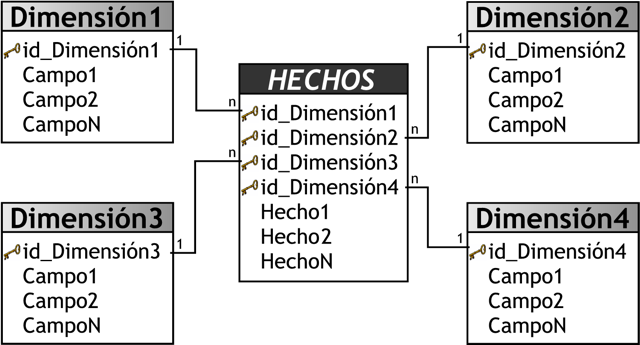
\includegraphics[width=10cm]{./Imagenes/1} 
\end{center}

\item Copo de Nieve
\begin{center}
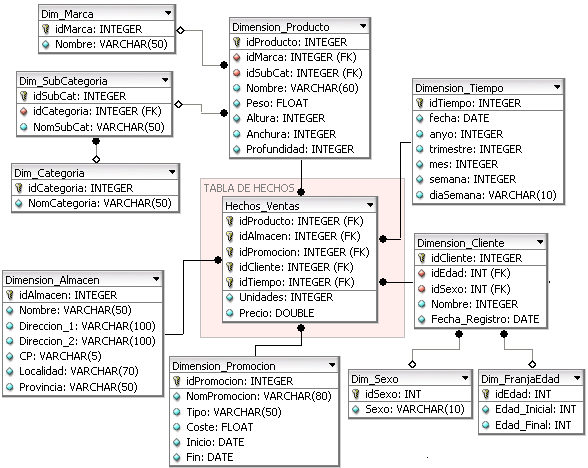
\includegraphics[width=10cm]{./Imagenes/2}
\end{center}


\item Constelacion
\begin{center}
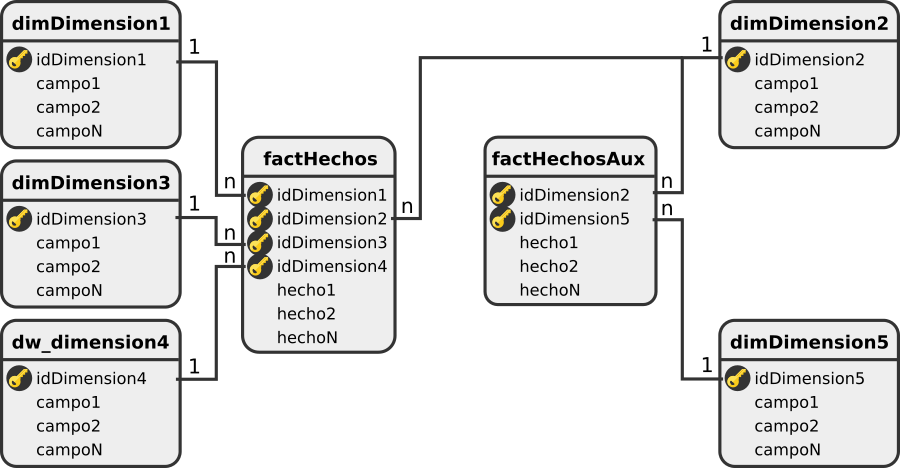
\includegraphics[width=10cm]{./Imagenes/3}
\end{center}

\subsection{Modelo Tabular}
	\item Los modelos tabular son base de datos de Analysis Services que se ejecutan en memoria o en modo DirectQuery(directo a la fuente). La base de datos que usaremos se descargar desde Github que es WorldWideImportersDW 

Todos los que hayan trabajado en Business Intelligence con las herramientas de Microsoft ya conocen lo que son los proyectos Multidimensionales de bases de datos. Son bases de datos hechas para la generación de reportes con un diseño especial muy diferente a las bases de datos transaccionales y con otro motor de base de datos.
Los modelos tabulares son bases de datos “en memoria” de Analysis Services. Gracias a los algoritmos de compresión avanzados y al procesador de consultas multiproceso, el motor analítico en memoria xVelocity (VertiPaq) ofrece un acceso rápido a los objetos y los datos de los modelos tabulares para aplicaciones cliente de reportes como Microsoft Excel y Microsoft Power View.
Los modelos tabulares admiten el acceso a los datos mediante dos modos: modo de almacenamiento en caché y modo DirectQuery. En el modo de almacenamiento en caché, puede integrar datos de varios orígenes como bases de datos relacionales, fuentes de distribución de datos y archivos de texto planos. En el modo DirectQuery, puede omitir el modelo en memoria, lo que permite a las aplicaciones cliente consultar los datos directamente en el origen relacional (SQL Server).
Analysis Services proporciona funciones de procesamiento analítico en línea (OLAP) y minería de datos para aplicaciones de Business Intelligence.
Los proyectos multidimensionales si bien les falta mucho para poder ser tan estables como las bases de datos transaccionales, están en una etapa más avanzada de desarrollo y grandes empresas ya lo utilizan.

Sugerencias:

\item  Primeramente, si ya se tiene una base de datos multidimensional, no se recomienda moverse a base de datos tabulares.
\item El hardware requerido para un proyecto tabular es muy diferente al requerido por un proyecto multidimensional. Por la compresión de datos, requiere menos disco una modelo tabular, pero requiere mucha más memoria RAM porque todo lo usa en memoria. En general, se necesita un buen CPU y memoria.
\item Los modelos tabulares consumen muchos recursos, por lo que se recomienda hacer pruebas del funcionamiento en un servidor de desarrollo y no en producción.
\item Se puede tener un modelo tabular y uno multidimensional instalados en la misma máquina, pero no es recomendable hacerlo en producción.

Ventajas del modelo tabular:

\item Mucho más veloz en consultas.
\item No requiere generar Aggregations (agregaciones) por lo que se simplifica el tiempo de procesamiento.
\item Gracias al DAX (el lenguaje para acceder a los datos equivalente al MDX), tiene mayor flexibilidad para obtener información.
\item Es intuitivo por lo que es mucho más rápido y fácil de entender e implementar.
\item Se basa en modelos relacionales.

Desventajas del modelo tabular:

\item  Las particiones no se procesaban en paralelo si no secuencialmente, lo que hace que sea más lento el procesamiento.
\item No se pueden usar multiples idiomas.
\item Si son muchos datos tarda bastante en manejar configuraciones de diferentes particiones.
\item El modelo tabular acapara demasiada memoria RAM y a su vez es dependiente de tal que afectará a otras aplicaciones.

Formato transaccional

Los datos transaccionales tienen un registro diferente para cada transacción o elemento. Si un cliente realiza varias compras, por ejemplo, cada una sería un registro diferente, con elementos asociados vinculados por un ID de cliente. Esto a veces se conoce como formato anidado.

\begin{center}
	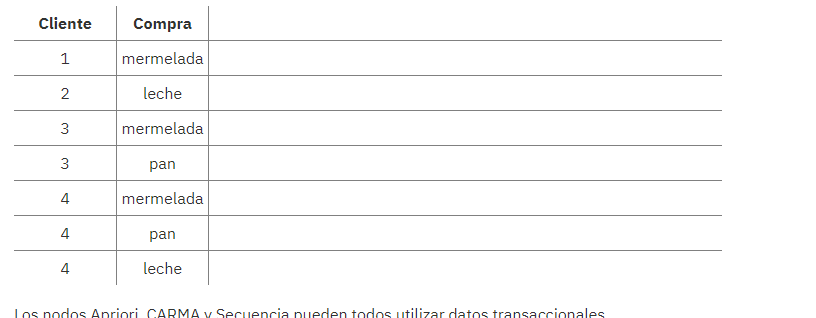
\includegraphics[width=10cm]{./Imagenes/33} 
\end{center}

Datos tabulares

Los datos tabulares (también conocidos como datos de la cesta o de la tabla de verdad) tienen elementos representados por marcadores diferentes, donde cada campo de marcas representa la presencia o ausencia de un elemento específico. Cada registro representa un conjunto completo de elementos asociados. Los campos de marcas pueden ser categóricos o numéricos, aunque ciertos modelos pueden tener requisitos más específicos.

\begin{center}
	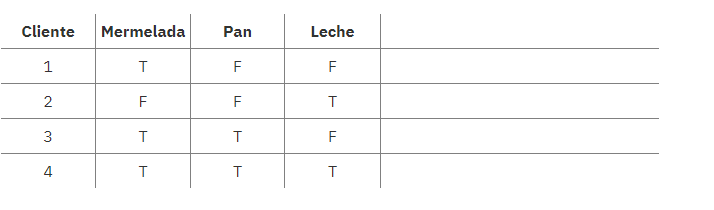
\includegraphics[width=10cm]{./Imagenes/22} 
\end{center}



\end{itemize}
\section{Conclusiones} 

\begin{itemize}
	\item Los modelos permiten ver las base de datos de otra forma de comprension haciendolas intuitivas para los usuarios no expoertos en el tema.
	\item En un almacén de datos el tiempo es muy importante y define la dinámica del negocio asociada a su jerarquía, la granularidad o nivel de detalle de la misma el tiempo es considerado una dimensión del almacén.
	\item Los diagramas de los demonios son de gran variedad y cada uno tiene un proposito especifico como normalizar estas tablas y reducir el espacio de almacenamiento al eliminar la redundancia.

\end{itemize} 

\section{Referencias} 

\subsection {Referencias}

\begin{itemize}
	\item L

\end{itemize} 



\end{document}
